\section{The \ara{} Protocol}
\label{sec:protocol}

The Agent-Native Research Artifact (\ara{}) protocol defines a file-system ontology that transforms CS research from a narrative document into a machine-executable knowledge package.
We describe the design philosophy (\S\ref{sec:philosophy}) and the layered architecture (\S\ref{sec:layers}).
Figure~\ref{fig:lrm-overview} (\S\ref{sec:live-pm}) illustrates how the Live Research Manager mediates between the human--AI research process and the living artifact across a long time horizon.


\begin{figure}[!t]
    \centering
    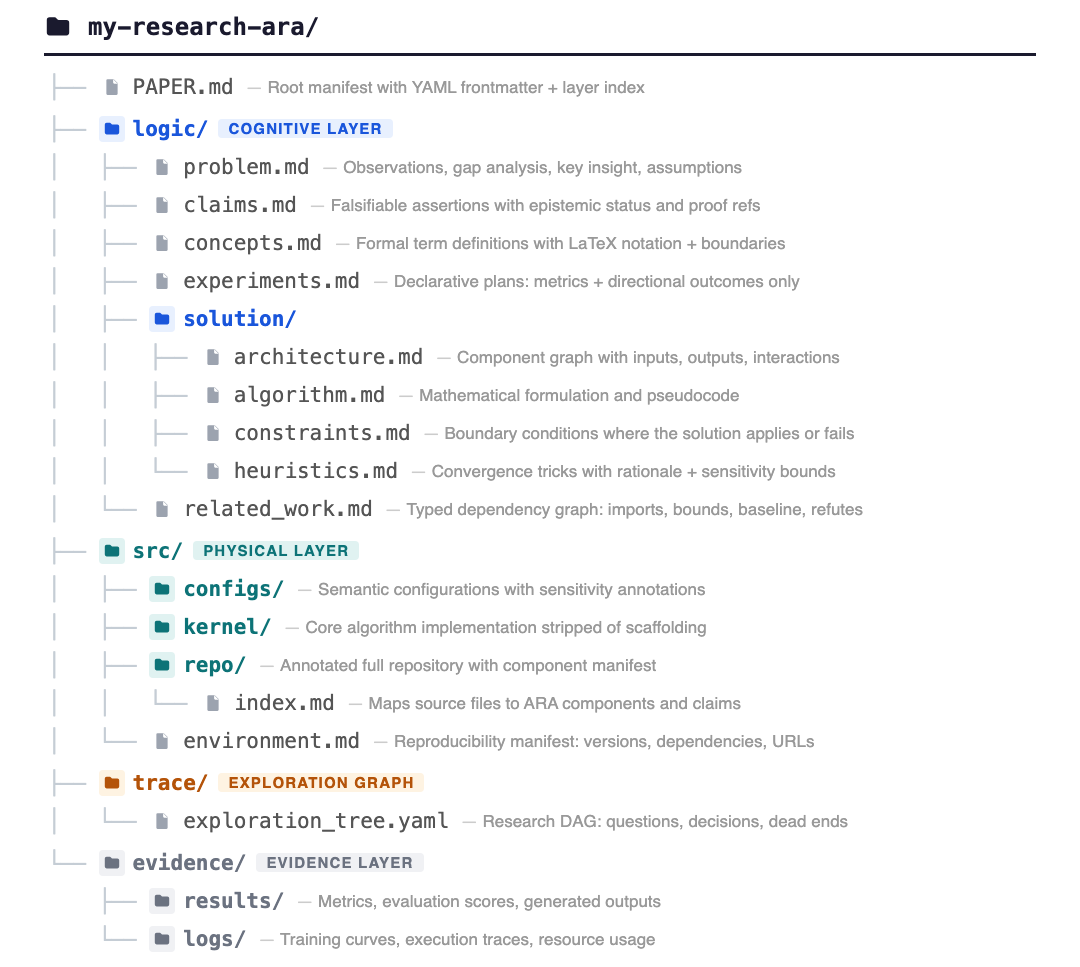
\includegraphics[width=\linewidth]{figures/fig_ara_directory_annotated.png}
    \caption{The \ara{} directory structure. Each file's role is annotated inline; layer badges mark the four top-level divisions. Cross-layer \emph{forensic bindings} link claims in \texttt{/logic} to evidence in \texttt{/evidence} and code in \texttt{/src}. Full schema in Appendix~\ref{app:schema}; design rationale in Appendix~\ref{app:protocol-details}.}
    \label{fig:ara-structure}
\end{figure}



\subsection{Design Philosophy}
\label{sec:philosophy}

The \ara{} protocol is grounded in a single principle: \textbf{Knowledge over Narrative}---the organized, evolving knowledge produced during research is the primary scientific object; the narrative paper is a compiled view.

\paragraph{A structured knowledge vessel.}
An agent engaging with a research project asks four structurally distinct questions: \emph{why} does this work (scientific reasoning), \emph{how} is it implemented (executable code), \emph{what was tried} along the way (exploration trajectory), and \emph{what are the numbers} (raw empirical evidence).
A narrative paper forces the agent to extract all four answers from the same linear prose, yet these knowledge types conflict in structure: reasoning demands stable, citable units while code iterates continuously; the exploration history is inherently branching while narrative enforces linearity; evidence requires machine-precise values while prose rounds and paraphrases.
Compressing them into a single document is not merely suboptimal but \emph{lossy}: once flattened into narrative, the original structure cannot be recovered.
\ara{} eliminates this loss by materializing each knowledge type as its own layer within an agent-native file-system structure (Figure~\ref{fig:ara-structure}): plain-text, independently queryable directories that agents navigate, read, and act on with standard tool calls, without parsing prose or reverse-engineering repositories.
Because agent context windows are a shared, finite resource, the structure further supports \emph{progressive disclosure}: agents load only the layers and files relevant to their current task, avoiding unnecessary context pollution.

The four layers below are the structural response to the Storytelling and Engineering Taxes introduced in \S\ref{sec:intro}: the Exploration Graph recovers the branching trajectory collapsed by narrative; the Cognitive and Physical Layers, bound by forensic links, close the gap between conceptual description and executable specification.
Within each layer, artifact text maximizes information per token: subjective qualifiers, hedges, and narrative connectives are stripped, and statements requiring judgment carry provenance rather than rhetoric.



\begin{figure}[!t]
    \centering
    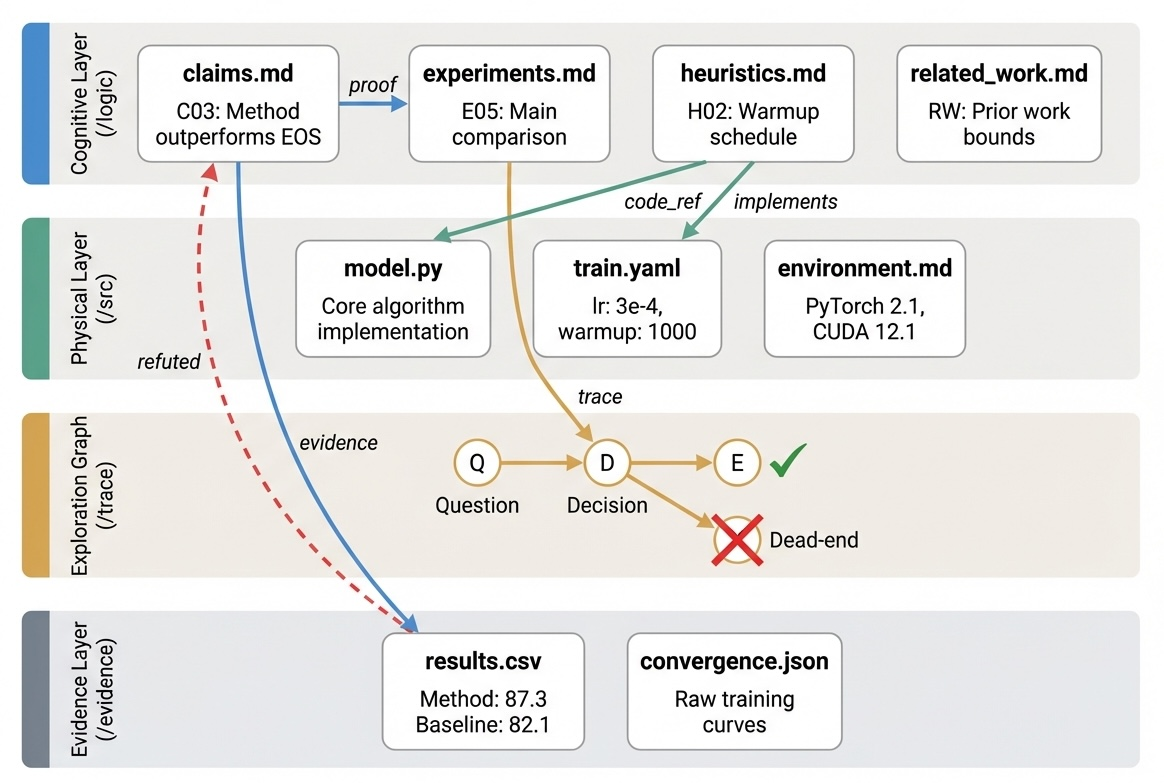
\includegraphics[width=\linewidth]{figures/fig_cross_layer_v2_attempt1.png}
    \caption{Cross-layer structure of a real \ara{}. Claims in \texttt{/logic} link to code in \texttt{/src} and evidence in \texttt{/evidence} via forensic bindings. The Exploration Graph (bottom center) captures the research DAG with dead-end nodes (marked $\times$) that preserve failure modes and lessons.}
    \label{fig:exploration-graph}
    \end{figure}
    
\subsection{\ara{} Architecture}
\label{sec:layers}

An agent engaging with a research artifact has four fundamental needs: \emph{understand} the contribution, \emph{reproduce} it, \emph{learn from the process}, and \emph{verify} claims against raw evidence.
\ara{} materializes each need as a dedicated layer (Figure~\ref{fig:ara-structure}), rooted in a manifest \texttt{PAPER.md} whose YAML frontmatter and layer index enable an agent to triage relevance in ${\sim}500$ tokens (Appendix~\ref{app:schema}).
The decomposition is informed by a taxonomy of ten reproduction-critical information categories derived from PaperBench rubrics (Appendix~\ref{app:taxonomy}).

\paragraph{The Cognitive Layer (\texttt{/logic}).}
An agent reads \texttt{/logic} \emph{first} to understand \emph{what was done and why}: \texttt{problem.md} defines the gap and key insight, \texttt{solution/} specifies the architecture, algorithm, and convergence-critical heuristics, \texttt{claims.md} distills falsifiable assertions with explicit proof pointers, and \texttt{experiments.md} declares the verification plan.
\texttt{related\_work.md} replaces passive citations with \emph{typed dependencies} that agents can act on: \texttt{imports} inject prior definitions, \texttt{bounds} propagate constraints to hyperparameter search, and \texttt{baseline} entries enable automatic regression detection, transforming literature review into a machine-executable dependency graph.

\paragraph{The Physical Layer (\texttt{/src}).}
Contains the \emph{how}---executable code calibrated to the contribution type.
Algorithmic contributions use \emph{kernel mode}: only the core modules with typed I/O signatures, often one to two orders of magnitude smaller than the full repository, so that a coding agent can regenerate environment-native boilerplate on demand.
Systemic contributions (CUDA kernels, distributed training, systems architectures) use \emph{repository mode}: the full implementation is retained but annotated via an \texttt{index.md} manifest that maps each source file to the \ara{} component it implements.
\texttt{configs/} annotates every hyperparameter with rationale and search range; \texttt{environment.md} pins dependencies, hardware, and seeds (mode specification, forensic bindings, and detailed rationale in Appendix~\ref{app:src-modes}).

\paragraph{The Exploration Graph (\texttt{/trace}).}
\texttt{exploration\_tree.yaml} stores the complete research directed acyclic graph (DAG) as a nested YAML tree with five typed node kinds---\texttt{question}, \texttt{decision}, \texttt{experiment}, \texttt{dead\_end}, \texttt{pivot}---where nesting encodes parent$\to$child edges and an \texttt{also\_depends\_on} field captures convergence points.
The format functions as a ``git log for research'': agents traverse branches directly, and dead-end nodes preserve the hypothesis, failure mode, and lesson that narrative papers discard (Figure~\ref{fig:exploration-graph}).

\paragraph{The Evidence Layer (\texttt{/evidence}).}
The raw outputs that ground every claim: \texttt{results/} contains machine-readable metric tables and generated data with exact values and source annotations; \texttt{logs/} captures training curves, resource usage, and diagnostics.
It holds \emph{outputs only}, so that every claim's proof chain flows \texttt{claims.md}\,$\to$\,\texttt{experiments.md}\,$\to$\,\texttt{/evidence/}.

\paragraph{Withholding ground-truth enables layered access control.}
Experiment \emph{logic} (what to verify) lives in \texttt{/logic}; experiment \emph{data} (exact results) lives exclusively in \texttt{/evidence}.
A verification agent can be granted the code kernel and algorithm descriptions while the evidence layer is withheld, preventing fabrication by copying expected values.
This separation also makes every \ara{} a ready-to-use training environment: the task lives in \texttt{/logic/experiments.md}, the reward in \texttt{/evidence/}, and preference signals in every accept, reject, and revision logged in \texttt{/trace/}.

We consider an \ara{} sufficient when a \emph{sufficiently capable} coding agent can reproduce the core claim \emph{zero-shot} from it, without human intervention or external context beyond the artifact itself. Sufficiency is therefore a capability-relative criterion: it measures whether the artifact \emph{contains} the information required to reproduce its claim, not whether any present-day agent can fully exploit it. At the limit of agent capability, a complete \ara{} is reproducible by definition, so artifacts authored today remain valid as agents advance.

